\section{Estado del arte}
\subsection[Búsqueda Scopus]{Búsqueda Scopus}
\begin{frame}
    \frametitle{Tendencia Scopus}
    \begin{columns}
      \column{0.6\textwidth}
    \begin{enumerate}
      \item \textbf{No hay muchas publicaciones}, aunque sí una tendencia positiva.
        \begin{itemize}
          \item Tampoco hay muchos datasets con altura de las personas etiquetados.
        \end{itemize}
      \item La tarea consiste en intentar medir en escala absoluta (en metros).
        \begin{itemize}
          \item Factores importantes: \textbf{contenido, contraste y distorsiones}.
          \item Objetivo: explotar ciertas invariantes geométricas.
        \end{itemize}
    \end{enumerate}
    \column{0.4\textwidth}
    \begin{figure}
      \begin{center}
        
\includegraphics[width=\textwidth]{imagenes/chapter1/Scopus-Analyze-Year}
      \end{center}
      \caption{Tendencia de publicaciones en el campo según Scopus.}
    \end{figure}
  \end{columns}
  \vspace{-.2cm}
\end{frame}
\note{
  La metrología de vista única, como se mencionaba anteriormente, está captando cada vez más atención, véase la Figura de publicaciones relacionadas sacada de Scopus.
  La tendencia es positiva, aunque sean pocos los números de artículos publicados.
  Esto puede que esté relacionado con las dificultades del campo y la poca disponibilidad de datos etiquetados con alturas reales.
  Hay varios factores que afectan a las estimaciones: problemas lumínicos, escenas con poca información geométrica o las distorsiones en la escena.
}
\subsection{Estado del arte}
\begin{frame}
    \frametitle{Fundamentos}
    \begin{columns}
      \column{0.5\textwidth}
      \begin{enumerate}
        \item Una parte fundamental del procedimiento consiste en la calibración de cámara~\footnotemark.
        \begin{enumerate}
        \item Utilizando un patrón geométrico conocido.
        \item Búsqueda de invariantes.
        \item Auto-calibración multi-vista.
        \end{enumerate}
      \item Permite eliminar distorsiones\footnotemark.
      \item Depende de la precisión y no siempre es generalizable.
      \end{enumerate}
      \column{0.5\textwidth}
      \begin{figure}
        \begin{center}
          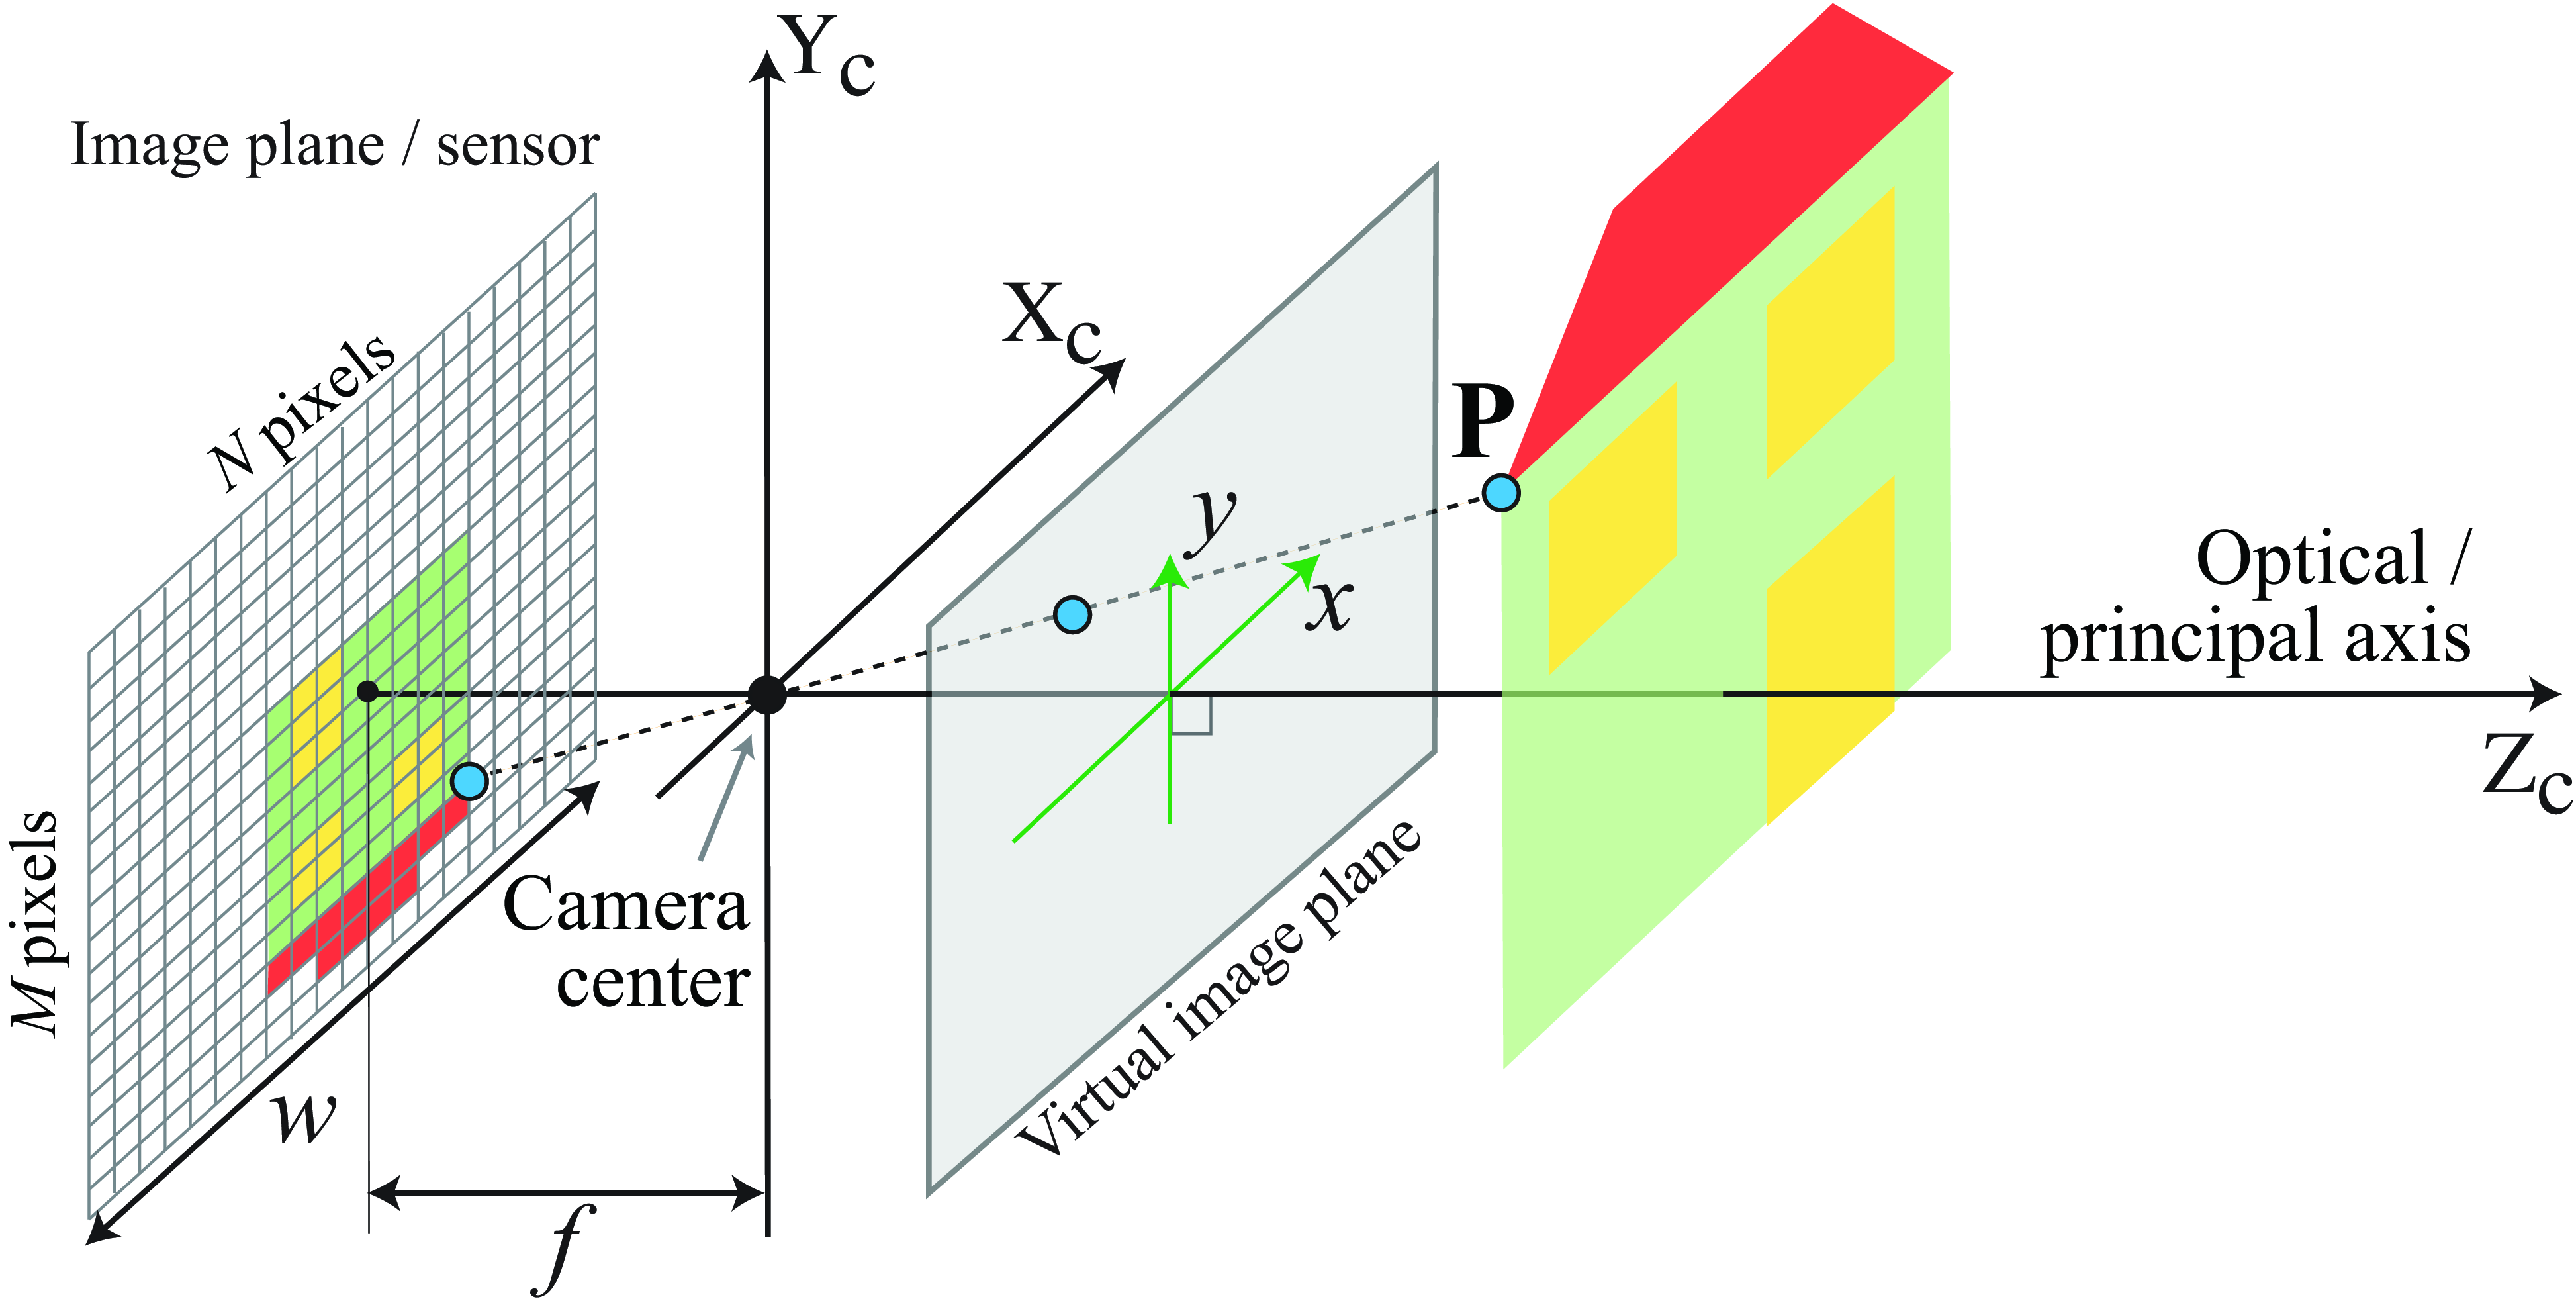
\includegraphics[width=0.9\textwidth]{imagenes/chapter2/pinhole_and_sensor.png}
        \end{center}
        \caption{Modelo de proyección de cámara.}
      \end{figure}
  \end{columns}
    \footcitetext{CalibrationSurvey}
    \footcitetext{VisionBookMIT}
\end{frame}

\note{
  Por eso, una parte fundamental del procedimiento significa entender cómo funciona la proyección 2D-3D.
  Para ello, es necesario conocer ciertos parámetros proyectivos de nuestra cámara. Se pueden obtener mediante un proceso llamado calibración.
  Al calibrar, se conoce la distancia focal, las distorsiones radiales de la lente y el punto principal.
  Hay varias formas para realizar la calibración, la mayoría de procesos son tediosos y manuales, como moverse por la escena con un patrón de ajedrez cuya geometría se conoce y
  se procura conservar durante la proyección.
  Para preserva dichas características, los parámetros estimados permiten rectificar la imagen, eliminando posibles distorsiones de lente.
  La limitación es que depende de la precisión de los algoritmos que obtienen dichos parámetros y los tipos de escenas, siendo no siempre generalizables.
}

\begin{frame}
  \frametitle{Métodos clásicos}
    \begin{columns}
    \column{0.5\textwidth}
    \begin{enumerate}
      \item Criminisi \emph{et al.}   sentó las bases metodológicas~\footnotemark.
      \item Describe técnicas para extracción de información geométrica.
        \begin{itemize}
          \item Ratio cruzado
        \end{itemize}
      \item Diversos autores extendieron sus trabajos.
    \end{enumerate}
    \column{0.5\textwidth}
    \begin{figure}
      \begin{center}
        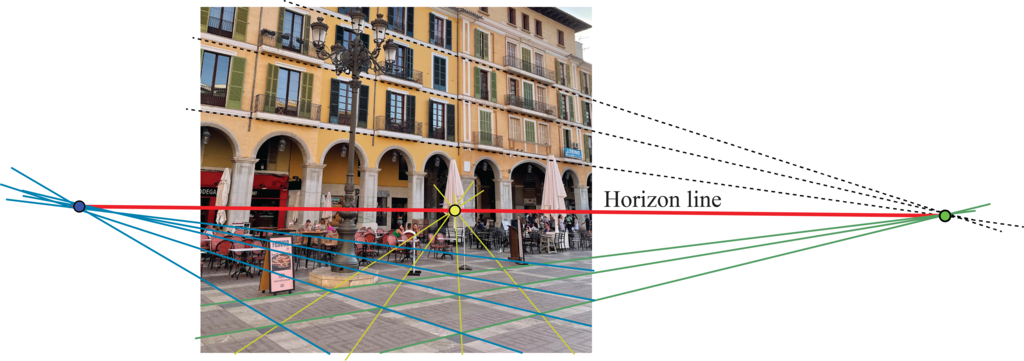
\includegraphics[width=1.1\textwidth]{imagenes/chapter2/palma_horizon.png}
      \end{center}
      \caption{Ejemplo de extracción de información geométrica~\footnotemark}
    \end{figure}
  \end{columns}
  \addtocounter{footnote}{-1}
  \footcitetext{CriminisiApplications, CriminisiPaintings, CriminisiReconstruction}
  \stepcounter{footnote}
  \footcitetext{VisionBookMIT}
\end{frame}

\note{
  Una vez entendido el modelo proyectivo, con los trabajos seminales de Criminisi et al. se tiene las bases metodológicas para metrología monocular.
  Sus trabajos han sido extendidos por diversos autores.
  Un ejemplo sería la imagen a la derecha, donde se observa cómo se utiliza las líneas paralelas para estimar el horizonte
  a partir de sus puntos de fuga. O por ejemplo utilizando el ratio cruzado entre puntos colineales para la estimación de la altura utilizando un objeto de referencia.
  No obstante, requiere saber alguna medida métrica de referencia de la escena.
}

\begin{frame}
  \frametitle{Aprendizaje profundo}
  \begin{enumerate}
    \item El aprendizaje profundo alcanza increíbles resultados en diversos campos.
    \item Existen diversos métodos para la calibración automática de escena.
    \item Combinan principios geométricos con modelos de aprendizaje~\footnotemark.
  \end{enumerate}
  \footcitetext{SVMIW}
\end{frame}
\note{
  Aquí es donde destacan los métodos de aprendizaje profundo. Estos aprenden a comprimir la información y características de
  grandes conjuntos de datos, para extrapolar e inferir sobre datos no vistos.
  Se han observado grandes avances en clasificación, estimación de profundidad y ahora en metrología monocular.
  Mediante la combinación de estos métodos de extracción automática de información y principios geométricos se consiguen métodos como el se verá a continuación.
  Por ello, el enfoque implementado será el mismo que en el artículo de Zhu et al.
  Aunque fue propuesto en 2020, resulta de especial interés al abordar
  específicamente la estimación métrica de objetos y de forma semi-supervisada,
  combinando aprendizaje con restricciones geométricas interpretables.
}
